\chapter{Cadre technique et développement}

\section{Introduction}
Ce chapitre présente le cadre technique du projet. Nous détaillons dans un premier temps l'environnement de travail et les outils utilisés, puis les technologies mobilisées pour le développement de la solution. Nous exposons ensuite l'architecture globale du système ainsi que les besoins fonctionnels et non fonctionnels ayant guidé sa conception, avant de conclure sur la cohérence de l'ensemble.

\section{Environnement de travail}

\subsection{Outils de scripting et d'automatisation}
\textbf{PowerShell} : des scripts (\texttt{.ps1}) ont été utilisés pour le lancement automatisé des différents services du projet.

\begin{figure}[H]
    \centering
    
\includegraphics[width=0.2\linewidth]{images/powersell_logo.jpeg}
    \caption{PowerShell}
    \label{fig:powershell}
\end{figure}

\subsection{Outils de test}
\textbf{pytest} : framework de tests unitaires et d'intégration utilisé pour la partie Python du projet.

\begin{figure}[H]
    \centering
    
\includegraphics[width=0.2\linewidth]{images/pytest_logo.png}
    \caption{pytest}
    \label{fig:pytest}
\end{figure}

\section{Technologies utilisées}

\subsection{Frontend}
\begin{itemize}
    \item \textbf{Next.js (15.x)} : framework React utilisé pour construire l'interface utilisateur dynamique et responsive, avec rendu côté serveur (SSR) et génération statique (SSG).
\begin{figure}[H]
    \centering
    
\includegraphics[width=0.2\linewidth]{images/next-js-logo.png}
    \caption{Next.js}
    \label{fig:nextjs}
\end{figure}
    \item \textbf{React (19.x)} : bibliothèque utilisée pour la conception de l'interface à base de composants.
\begin{figure}[H]
    \centering
    
\includegraphics[width=0.2\linewidth]{images/react.png}
    \caption{React}
    \label{fig:react}
\end{figure}
    \item \textbf{TypeScript (5.7.x)} : sur-ensemble typé de JavaScript garantissant un code plus fiable et maintenable.
\begin{figure}[H]
    \centering
    
\includegraphics[width=0.2\linewidth]{images/typescript.png}
    \caption{TypeScript}
    \label{fig:typescript}
\end{figure}
    \item \textbf{Tailwind CSS (3.4.x)} : framework CSS utilitaire pour le stylage rapide de l'interface.
\begin{figure}[H]
    \centering
    
\includegraphics[width=0.2\linewidth]{images/tailwind.png}
    \caption{Tailwind CSS}
    \label{fig:tailwind}
\end{figure}
\end{itemize}

\subsection{Backend}
\begin{itemize}
    \item \textbf{FastAPI (0.115)} : framework Python utilisé pour exposer l'API REST et gérer la logique métier.
\begin{figure}[H]
    \centering
    
\includegraphics[width=0.2\linewidth]{images/fastapi.png}
    \caption{FastAPI}
    \label{fig:fastapi}
\end{figure}
    \item \textbf{Python} : gestion des variables d'environnement.
\begin{figure}[H]
    \centering
    
\includegraphics[width=0.1\linewidth]{img/python_ligo.png}
    \caption{Python}
    \label{fig:python}
\end{figure}
\end{itemize}

\subsection{Intelligence artificielle et orchestration agentique}
\begin{itemize}
    \item \textbf{LangGraph (0.2.34)} : orchestration de l'agent par graphe d'états.
\begin{figure}[H]
    \centering
    
\includegraphics[width=0.2\linewidth]{images/langgraph-logo-png.png}
    \caption{LangGraph}
    \label{fig:langgraph}
\end{figure}
    \item \textbf{LangChain (0.3.1)} : framework de développement d'applications basées sur les LLM.
\begin{figure}[H]
    \centering
    
\includegraphics[width=0.2\linewidth]{images/langchaine.png}
    \caption{LangChain}
    \label{fig:langchain}
\end{figure}
    \item \textbf{Ollama} : exécution locale des modèles de langage, avec \texttt{llama3.1:8b} pour la génération et \texttt{nomic-embed-text} pour les \textit{embeddings}.
\begin{figure}[H]
    \centering
    
\includegraphics[width=0.2\linewidth]{images/ollama_logo.png}
    \caption{Ollama}
    \label{fig:ollama}
\end{figure}
\end{itemize}

\paragraph{Fonctionnement d'Ollama dans le projet.}
Ollama est utilisé comme moteur de modèle de langage local (par défaut \texttt{llama3.2} ou \texttt{llama3.1:8b}), garantissant la confidentialité et la souveraineté totale des données d'entreprise, sans dépendance à une API Cloud payante. Ollama intervient à plusieurs étapes stratégiques du projet :
\begin{itemize}
    \item \textbf{Explication et justification du choix fournisseur :} l'algorithme mathématique calcule le score et classe les fournisseurs. Ensuite, Ollama reçoit ces métriques précises (scores, prix, délais, qualité) et génère une explication argumentée et synthétique en langage naturel (2 à 3 phrases) pour expliquer à l'acheteur pourquoi ce fournisseur a été choisi face à ses concurrents.
    \item \textbf{Synthèse et restitution en langage naturel :} transforme les données techniques brutes retournées par Business Central ou par le graphe en une réponse fluide, courtoise et professionnelle pour l'utilisateur, tout en conservant les tableaux et données clés.
    \item \textbf{Embeddings et RAG vectoriel :} utilisation du modèle d'embedding local \texttt{nomic-embed-text} via Ollama pour la recherche sémantique dans la documentation ou le catalogue article/fournisseur stocké dans Qdrant.
\end{itemize}

\subsection{ERP et intégration}
\begin{itemize}
    \item \textbf{Microsoft Dynamics 365 Business Central}
\begin{figure}[H]
    \centering
    
\includegraphics[width=0.2\linewidth]{images/business-central-logo.png}
    \caption{Microsoft Dynamics 365 Business Central}
    \label{fig:business-central}
\end{figure}
    \item \textbf{Docker} : conteneur Windows utilisé pour exécuter Business Central.
\begin{figure}[H]
    \centering
    
\includegraphics[width=0.2\linewidth]{images/docker_logo.png}
    \caption{Docker}
    \label{fig:docker}
\end{figure}
\end{itemize}

\section{Architecture et intégration}

\subsection{Besoins fonctionnels}
Les besoins fonctionnels correspondent aux fonctionnalités que l'application doit offrir aux utilisateurs :
\begin{itemize}
    \item \textbf{Interaction conversationnelle :} l'utilisateur doit pouvoir dialoguer en langage naturel avec l'agent pour formuler ses demandes (analyse de stock, recommandation de fournisseur, création de commande).
    \item \textbf{Analyse de stock :} le système doit permettre de consulter le niveau de stock des articles et d'identifier automatiquement ceux en rupture.
    \item \textbf{Classification d'intention :} l'application doit détecter automatiquement le type de demande formulée par l'utilisateur et orienter le traitement en conséquence.
    \item \textbf{Recommandation de fournisseur :} le système doit proposer un fournisseur adapté à un article donné, en s'appuyant sur un scoring multi-critères (prix, délai, qualité, fiabilité, historique).
    \item \textbf{Prévisualisation de commande :} l'utilisateur doit pouvoir consulter un récapitulatif (fournisseur, prix unitaire, quantité, coût total) avant toute validation.
    \item \textbf{Confirmation et création de commande :} la création effective d'une commande dans l'ERP doit être conditionnée par une validation explicite de l'utilisateur, et le document créé doit être enregistré en statut brouillon.
    \item \textbf{Continuité de service :} l'application doit basculer automatiquement sur des données locales en cas d'indisponibilité de l'ERP, de manière transparente pour l'utilisateur.
    \item \textbf{Configuration du scoring :} un utilisateur habilité doit pouvoir ajuster les pondérations des critères d'évaluation selon la stratégie d'achat souhaitée.
    \item \textbf{Tableau de bord :} l'application doit permettre de visualiser les scénarios d'évaluation, de déclencher le calcul du scoring et de générer la commande pour le fournisseur le mieux classé.
    \item \textbf{Historique des livraisons :} le système doit journaliser les événements de livraison afin d'affiner les évaluations futures des fournisseurs.
\end{itemize}

\subsection{Besoins non fonctionnels}
Les besoins non fonctionnels concernent la qualité et les contraintes de l'application :
\begin{itemize}
    \item \textbf{Fiabilité :} assurer la continuité du service via un mécanisme de reprise automatique (retry, circuit breaker) en cas d'indisponibilité de l'ERP.
    \item \textbf{Performance :} garantir des temps de réponse acceptables malgré les contraintes de concurrence imposées par le serveur ERP, notamment grâce à un cache local.
    \item \textbf{Sécurité et gouvernance :} empêcher toute création de commande sans validation humaine explicite, afin d'éviter tout engagement involontaire.
    \item \textbf{Traçabilité :} conserver un statut clair pour chaque commande (brouillon, ouvert) permettant une révision avant tout engagement définitif.
    \item \textbf{Disponibilité :} assurer un fonctionnement en mode dégradé en s'appuyant sur des données locales en cas de panne du système central.
    \item \textbf{Interopérabilité :} communiquer avec l'ERP via un protocole standard afin de rester compatible avec les évolutions futures de la plateforme.
    \item \textbf{Maintenabilité :} structurer l'architecture en couches découplées (interface, API, orchestration, connecteur de données) pour faciliter les évolutions.
    \item \textbf{Ergonomie :} proposer une interface simple et réactive, avec des actions rapides pour les opérations courantes.
    \item \textbf{Évolutivité :} permettre l'ajout de nouveaux critères de scoring ou de nouveaux scénarios sans remettre en cause l'architecture existante.
\end{itemize}

\subsection{Acteurs}

\textbf{Responsable des Achats :}
\begin{itemize}
    \item Demande des recommandations sur le meilleur fournisseur pour un article.
    \item Consulte les comparatifs (prix, délais, scoring qualité).
    \item Vérifie la prévisualisation du bon de commande et le valide (Human-in-the-Loop).
\end{itemize}

\textbf{Gestionnaire des Stocks :}
\begin{itemize}
    \item Interroge l'état des stocks et les ruptures imminentes en langage naturel.
    \item Analyse les tendances d'achat et les prévisions de demande future.
    \item Lance des alertes de réapprovisionnement.
\end{itemize}

\textbf{Comptable Fournisseurs :}
\begin{itemize}
    \item Suit les commandes d'achats en cours.
    \item Détecte les anomalies sur les factures et surveille les dépassements de budget.
    \item Valide les flux d'approbation financière.
\end{itemize}

\textbf{Administrateur Système :}
\begin{itemize}
    \item Configure la connexion avec Microsoft Dynamics 365 Business Central.
    \item Gère le multi-sociétés.
    \item Supervise les modèles Ollama et les services d'infrastructure.
\end{itemize}

\subsection{Synthèse des problèmes résolus}

\begin{table}[htbp]
\centering
\renewcommand{\arraystretch}{1.4}
\resizebox{\textwidth}{!}{%
\begin{tabular}{|p{6cm}|p{8cm}|}
\hline
\textbf{Problème réel en entreprise} & \textbf{Solution apportée par le projet} \\
\hline
Complexité et lourdeur des ERP (Business Central, SAP, etc.) &
Permet à n'importe quel collaborateur d'interagir avec l'ERP en langage naturel, sans devoir maîtriser les masques de saisie complexes. \\
\hline
Ruptures de stock imprévues &
Détection proactive des niveaux de stock critiques et calcul automatique des quantités à réapprovisionner. \\
\hline
Choix sous-optimal des fournisseurs &
Sélection objective et automatique du meilleur fournisseur via un scoring combinant prix, délai de livraison et fiabilité passée. \\
\hline
Erreurs de saisie manuelle de commandes &
Automatisation de la création des en-têtes et lignes de commandes dans l'ERP, avec prévisualisation et contrôle du total. \\
\hline
Peur de l'automatisation incontrôlée (sécurité) &
Principe du Human-in-the-Loop : aucune commande n'est validée sans accord explicite de l'utilisateur, les commandes restant en statut Brouillon. \\
\hline
Confidentialité des données d'achats &
Traitement local via Ollama et connecteurs locaux/on-premise, évitant la fuite de données financières sensibles vers des clouds tiers. \\
\hline
\end{tabular}%
}
\caption{Problèmes réels résolus par le projet}
\label{tab:problemes-resolus}
\end{table}

\subsection{Architecture globale du système}
\begin{figure}[h!]
    \centering
    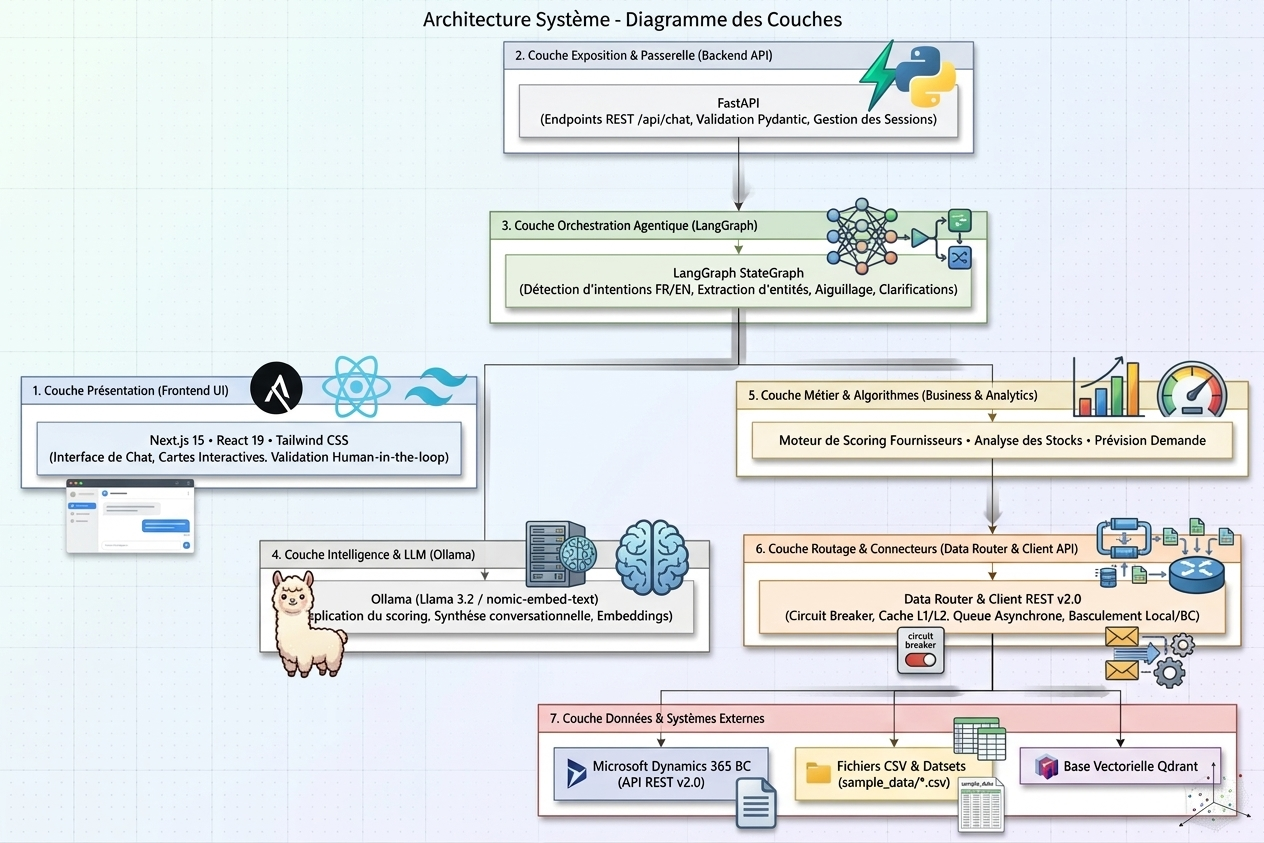
\includegraphics[width=1\linewidth]{images/Architecture_sys.png}
    \caption{Architecture globale du système}
    \label{fig:architecture}
\end{figure}

\section{Conclusion}
Ce chapitre a permis de poser le cadre technique du projet : environnement de travail, technologies retenues, besoins fonctionnels et non fonctionnels, acteurs impliqués et architecture globale du système. Ces éléments constituent le socle sur lequel repose la réalisation présentée dans le chapitre suivant.